\documentclass[]{article}
\usepackage{graphicx}
\usepackage[margin=1.25in]{geometry}



%% opening
\title{Mitacs Internship Report}
\author{Srivarshan Selvaraj}



\begin{document}



\maketitle



\begin{abstract}
The internship at the MacEwan University, under the guidance of Professor Cristina Anton, consisted of the study and experimentation with various model-based EM algorithms used to cluster contaminated functional data. The proposed algorithms, \emph{tfunHDDC} and \emph{cfunHDDC} were evaluated on benchmark datasets against some similar algorithms, \emph{funHDDC} and \emph{funclust}. The datasets used to benchmark the algorithms were the ECG and Kneading datasets. A new R package called \emph{tourr}, used for visualizing multidimensional data was also explored and used to explore the Chemical dataset. Finally, the \emph{Functional Isolation Forest} algorithm for detecting outliers in data was used to detect the outliers in both the ECG and Kneading data and also used as an clustering algorithm on the ECG data.
\end{abstract}



\section{Introduction}

Functional data analysis relates to the analysis and theory of data in the form of functions, surfaces or curves. Nowadays model based EM algorithms are quite prevalent in clustering of such functional data. But one situation were such algorithms may face issues is the clustering of real data which are often contaminated with outliers. These outliers affect the ability of the algorithms to properly estimate the model parameters. 

The cfunHDDC is an algorithm for clustering of functional data contaminated with mild outliers. This algorithm is based on the funHDDC algorithm to cluster functional data and the CNmixt method for multivariate data. The tfunHDDC algorithm differs from the cfunHDDC by using a t distribution instead of considering a mixed distribution with contamination. This results in longer tails, the length of which is decided by the degrees of freedom of the model. These models along with funHDDC were used to cluster the ECG and Kneading data and their performance was analysed.

The R package tourr is an implementation of the Tour methods for the visualization of multivariate data. It has been used to visualize the Chemical dataset to select the best concentrations and best components after PCA so that these can be used to cluster them. The Functional Isolation Forest algorithm is an extension of the popular Isolation Forest method for anomaly detection. This algorithm has been extended to detect the outliers in functional data. The algorithm can also be used to cluster data into two groups, provided that the proportion of the clusters is known beforehand, or it is a balanced dataset. This method has been used to detect the outliers present in both the ECG and Kneading data and to cluster the ECG data.



\section{Dataset}
Two main datasets have been used over the course of the internship; they are the ECG data and the Kneading data.

The ECG dataset is taken from the UCR Time Series Classification and Clustering website.The ECG data relates to the data recorded by 200 electrocardiogram from 2 groups of patients sampled at 96 time instants such readings that have been taken split between 2 files called "TRAIN" and "TEST". These two files were combined to create a single dataset with 200 readings. The readings were divided into two 2 classes, generalized as "Class 1" and "Class 2". Figure \ref{fig:ecg_data} shows the ECG data and its 2 classes.

\begin{figure}
	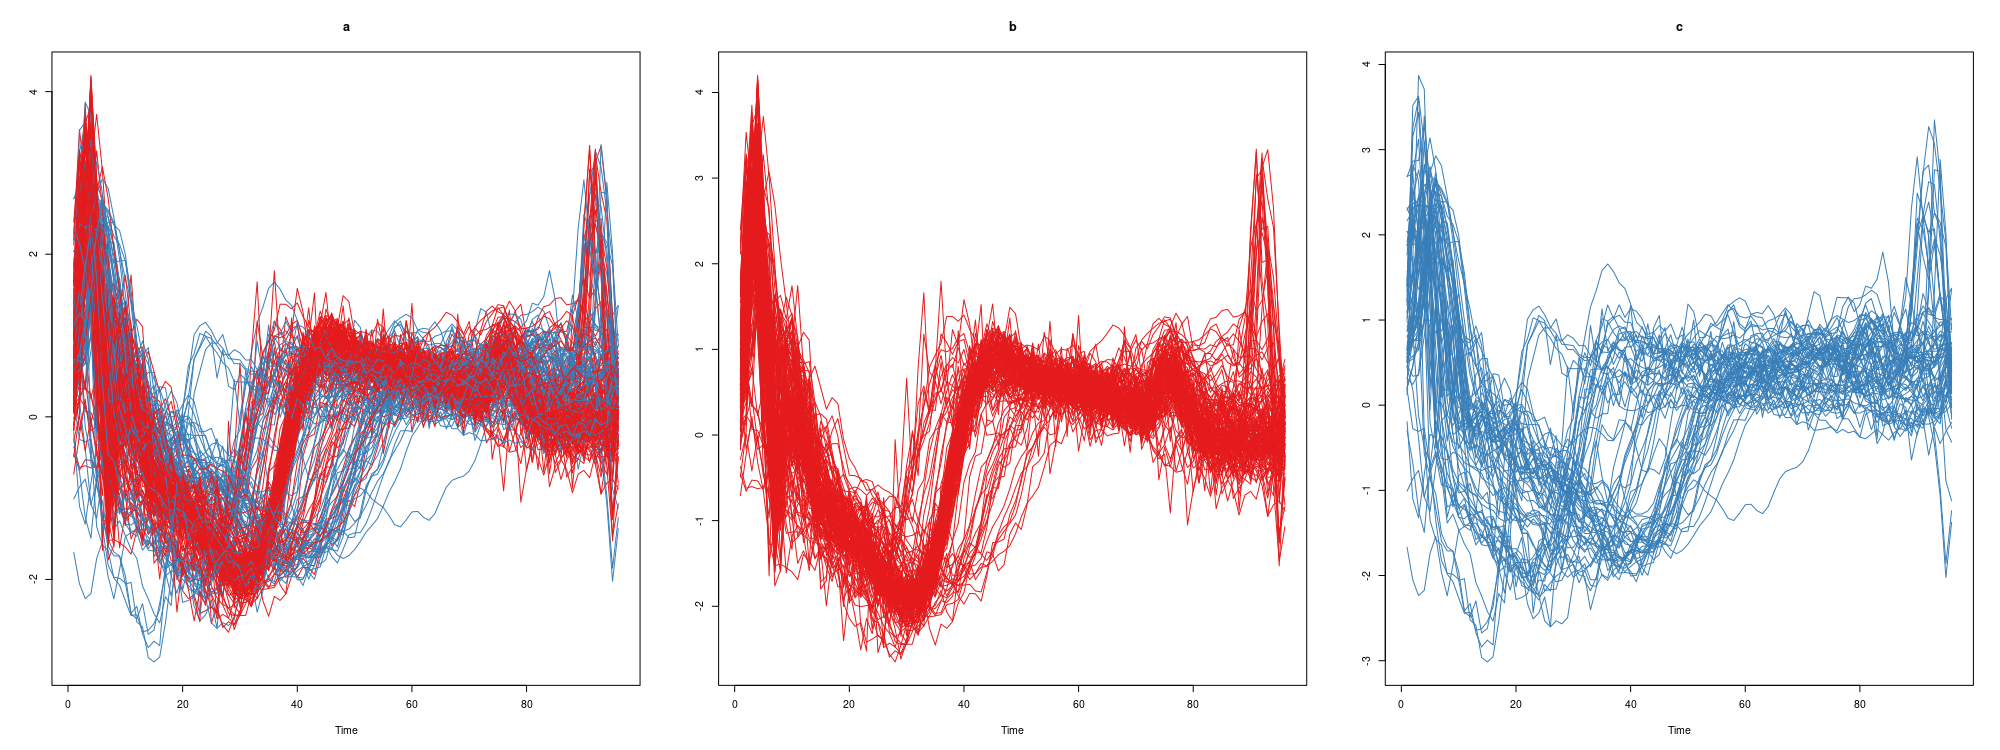
\includegraphics[width=\linewidth]{ecg_data.png}
	\caption{ECG Data.}
	\label{fig:ecg_data}
\end{figure}

The Kneading data comes from Danone Vitapole Paris Research Center and concerns the quality of cookies and the relationship with the flour kneading process. There are 115 different flours for which the dough resistance is measured during the kneading process for 480 seconds. One obtains 115 kneading curves observed at 241 equispaced instants of time. The 115 flours produce cookies of different qualities: 50 of them have produced cookies of good quality, 25 produced medium quality and 40 low quality. Figure \ref{fig:kneading_data} shows the Kneading data and its 3 classes.

\begin{figure}
	\centering
	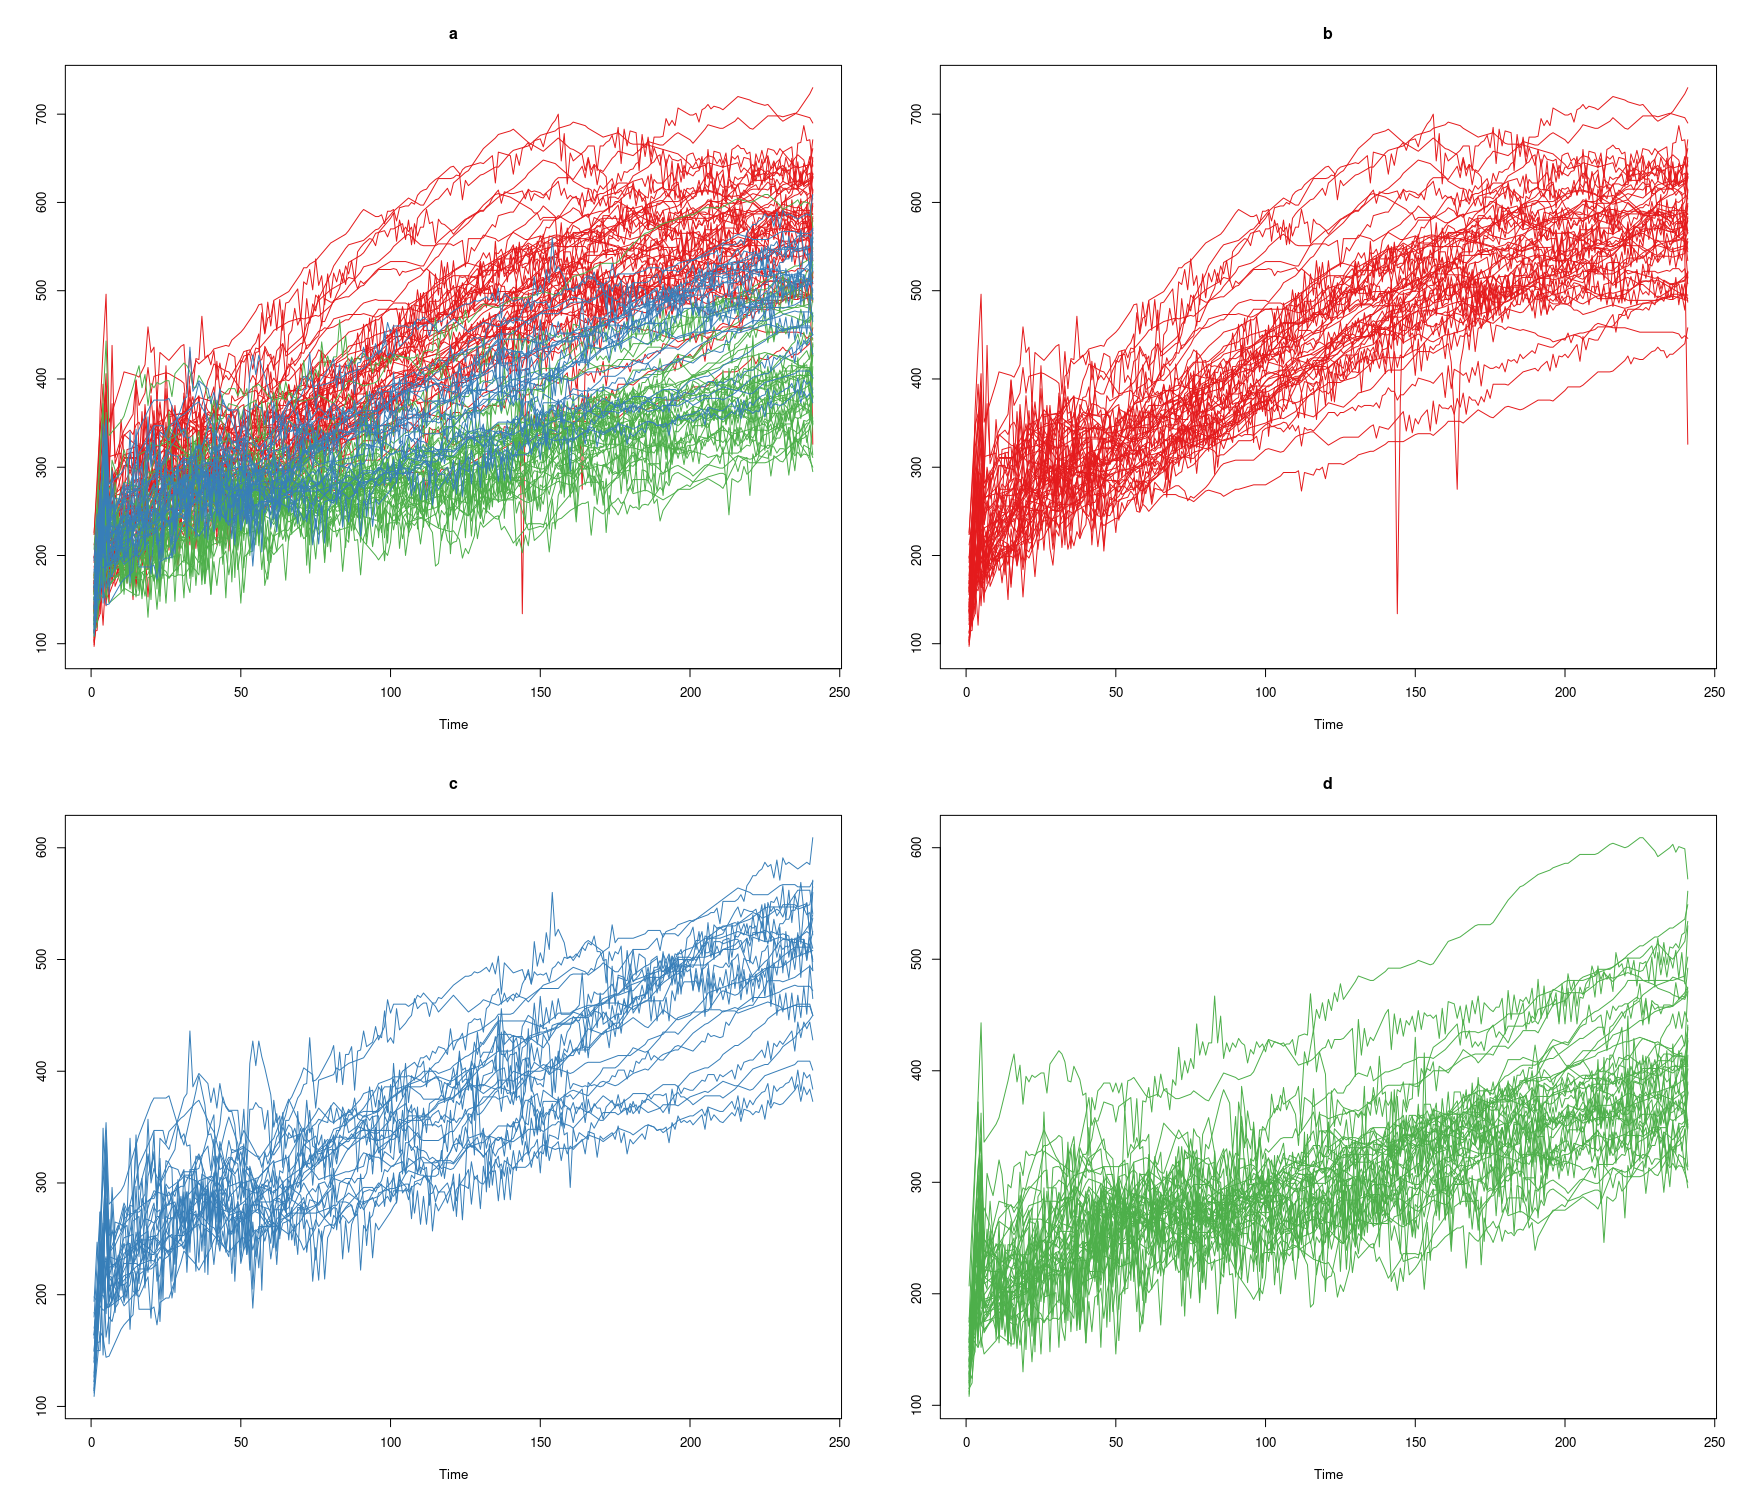
\includegraphics[scale=0.25]{kneading_data.png}
	\caption{ECG Data.}
	\label{fig:kneading_data}
\end{figure}



\section{Clustering of ECG Dataset}

The ECG data was converted into functional data by approximating it with both the Fourier and B-spline basis. However, since other benchmarks are only against curves creates using B-spline basis, the Fourier basis has been disregarded. The B-spline basis uses 20 splines to approximate the raw data. The outlier.depth.trim function in R was used to detect the outliers in the dataset, which turned out to be 5. This is a low amount of outliers, about 2.5\% of the entire data. All three clustering algorithms have various parameters that have to be fine-tuned to obtain the highest performance. Thus a gridsearch was performed by varying all the parameters to find the best performing method and its configuration. The results can be found in Table \ref{tab:ecg_data}.

\begin{table}
	\centering
	\begin{tabular}{c c c} 
		\hline
		Method & Configuration & CCR \\ [0.5ex] 
		\hline
		funHDDC & thresh 0.05 & 74.50 \\ 
		
		tfunHDDC & thresh 0.4; dfupdate numeric; dconstr yes & 75.50 \\
		
		cfunHDDC & thresh 0.05; alpha 0.85 & 74.50 \\ [1ex] 
		\hline
	\end{tabular}
	\caption{Performance of the algorithms on ECG data.}
	\label{tab:ecg_data}
\end{table}

The final cluster obtained by the best performing model tfunHDDC is shown in Figure \ref{fig:ecg_cluster}.

\begin{figure}
	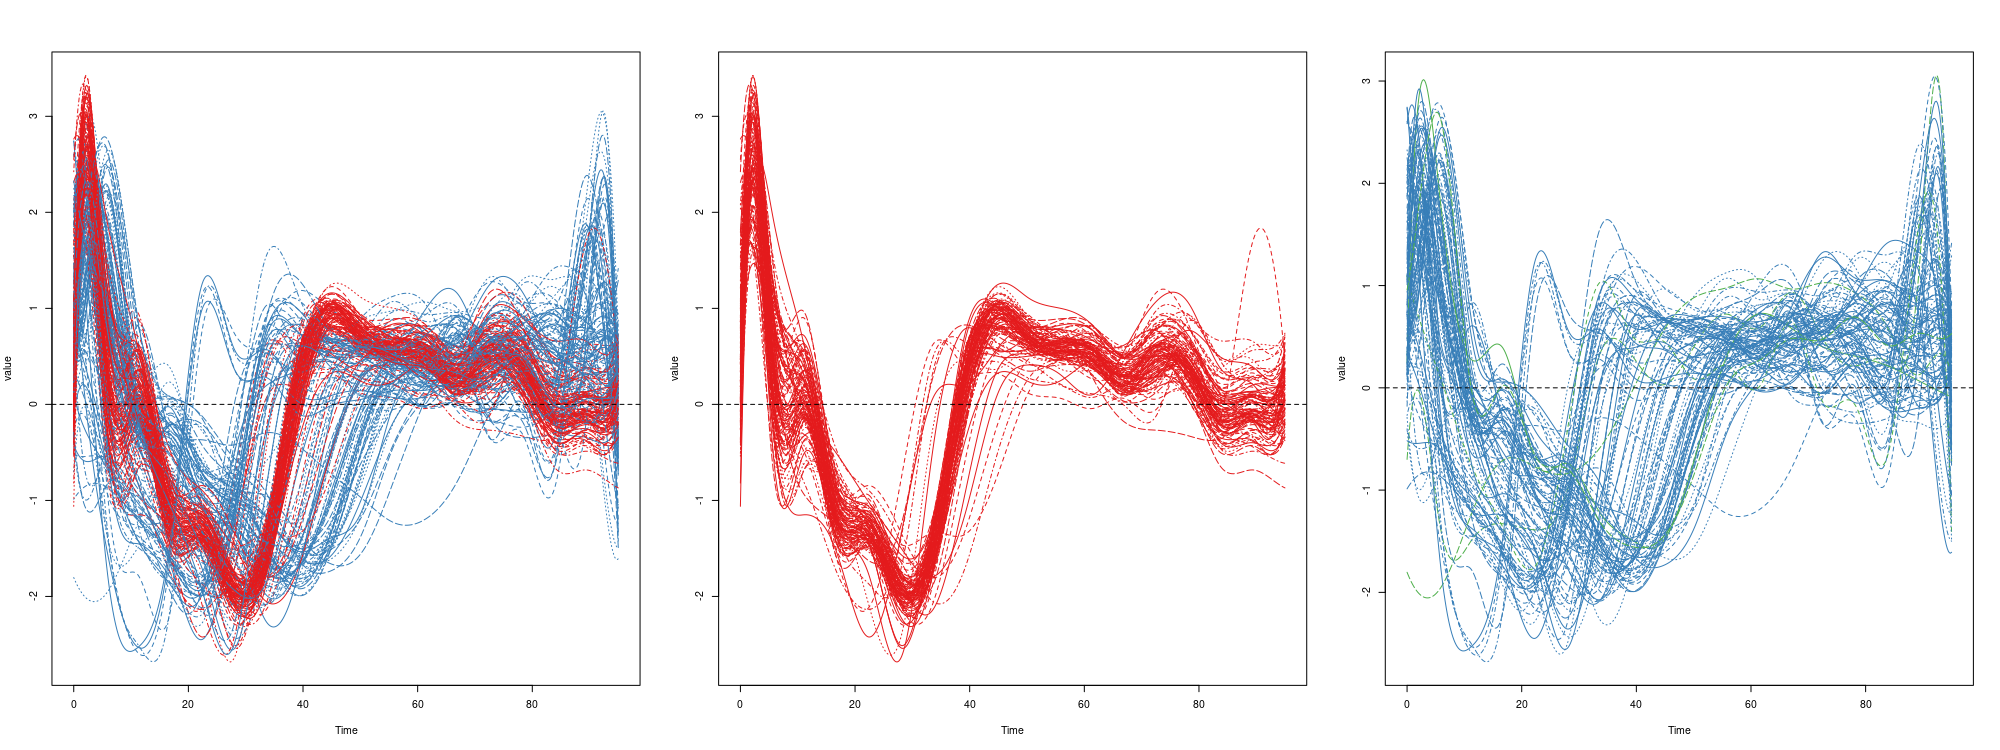
\includegraphics[width=\linewidth]{ecg_cluster.png}
	\caption{Clustering of ECG Data by tfunHDDC.}
	\label{fig:ecg_cluster}
\end{figure}



\section{Clustering of Kneading Dataset}

The kneading data was converted into functional data by approximating it with both the Fourier and B-spline basis. However, since other benchmarks are only against curves creates using B-spline basis, the Fourier basis has been disregarded. The B-spline basis uses 20 splines to approximate the raw data. The outlier.depth.trim function in R was used to detect the outliers in the dataset, which turned out to be 7. This is a medium amount of outliers, about 7.3\% of the entire data. All three clustering algorithms have various parameters that have to be fine-tuned to obtain the highest performance. Thus a gridsearch was performed by varying all the parameters to find the best performing method and its configuration. The results can be found in Table \ref{tab:kneading_data}.

\begin{table}
	\centering
	\begin{tabular}{c c c} 
		\hline
		Method & Configuration & CCR \\ [0.5ex] 
		\hline
		funHDDC & thresh 0.4 & 63.48 \\ 
		
		tfunHDDC & thresh 0.4 & 73.91 \\
		
		cfunHDDC & thresh 0.2, 0.3 or 0.4 & 70.43 \\ [1ex] 
		\hline
	\end{tabular}
	\caption{Performance of the algorithms on Kneading data.}
	\label{tab:kneading_data}
\end{table}

The final cluster obtained by the best performing model tfunHDDC is shown in Figure \ref{fig:kneading_cluster}.

\begin{figure}
	\centering
	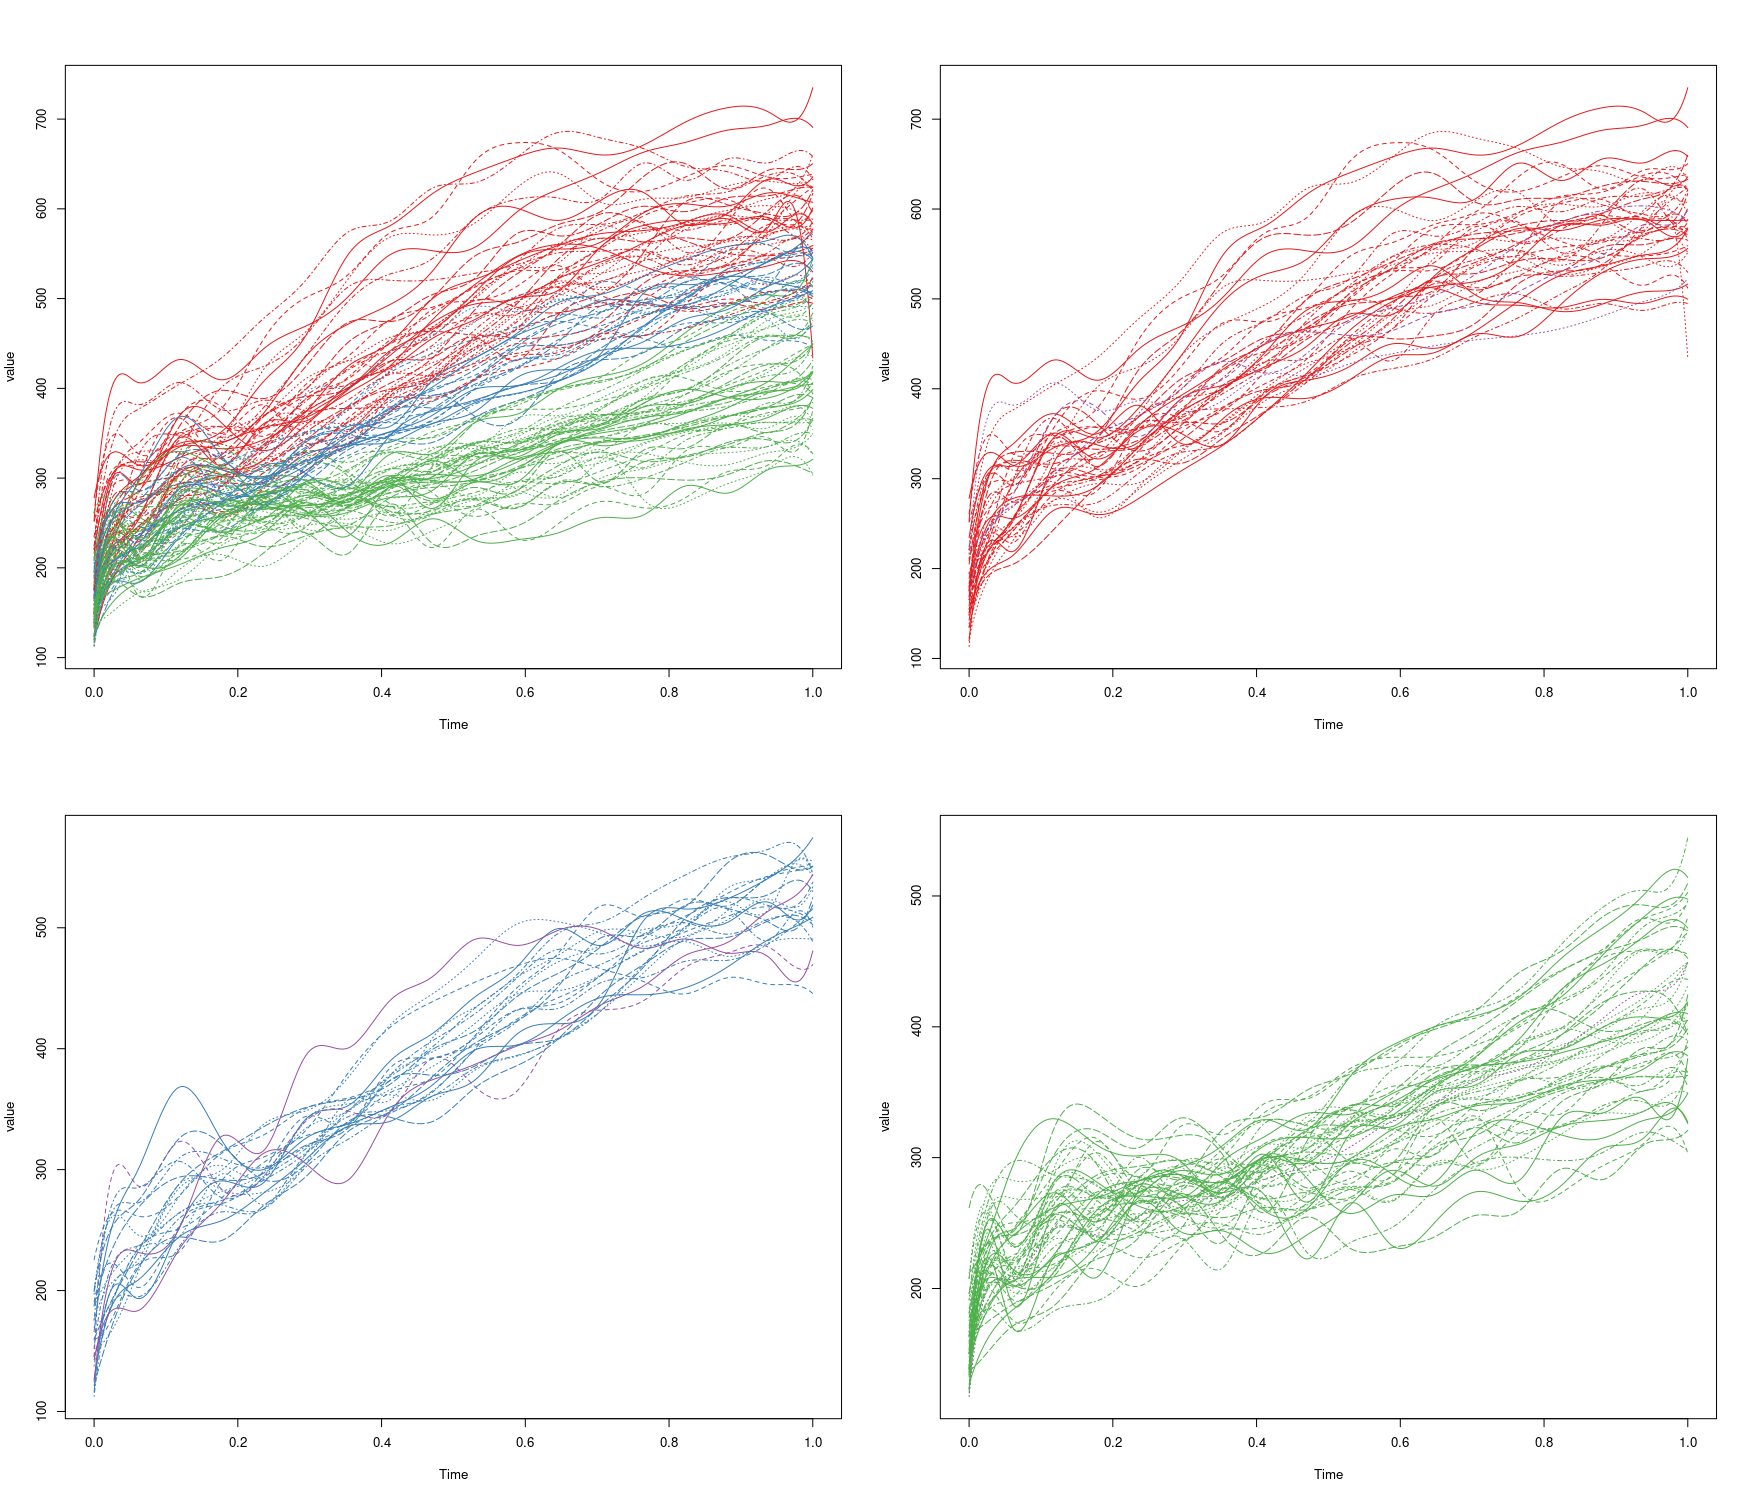
\includegraphics[scale=0.25]{kneading_cluster.png}
	\caption{Clustering of Kneading Data by tfunHDDC.}
	\label{fig:kneading_cluster}
\end{figure}



\section{Visualization of Multivariate Data}

The R package \emph{tourr} was used to visualize the multivariate chemical data. Both the PCA and the splines were analysed to see which components give the maximum separation so that they can be included in the clustering algorithms. Some of the visualizations obtained are given in Figures \ref{fig:pca_10} and \ref{fig:spline_10}.

\begin{figure}
	\centering
	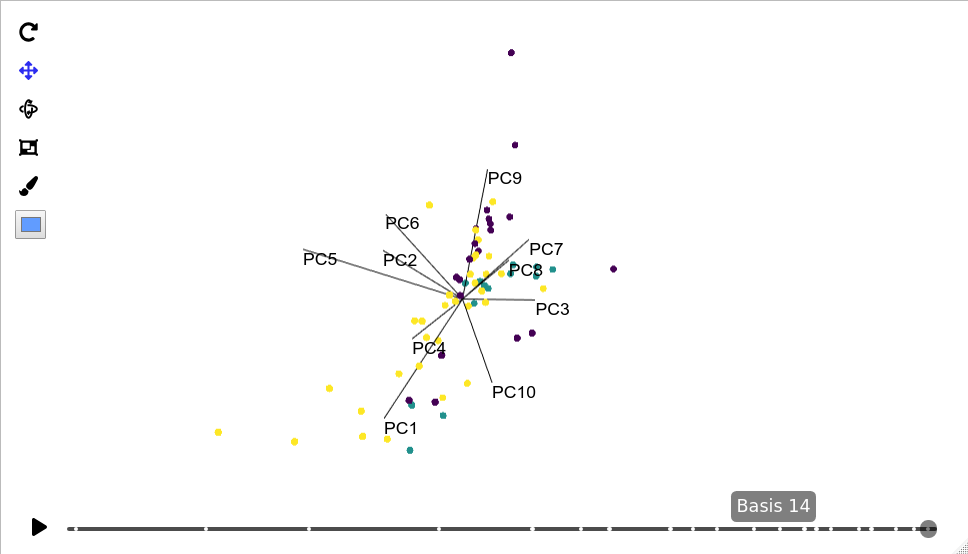
\includegraphics[scale=0.35]{pca_10.png}
	\caption{Visualization of 10th component of the PCA.}
	\label{fig:pca_10}
\end{figure}

\begin{figure}
	\centering
	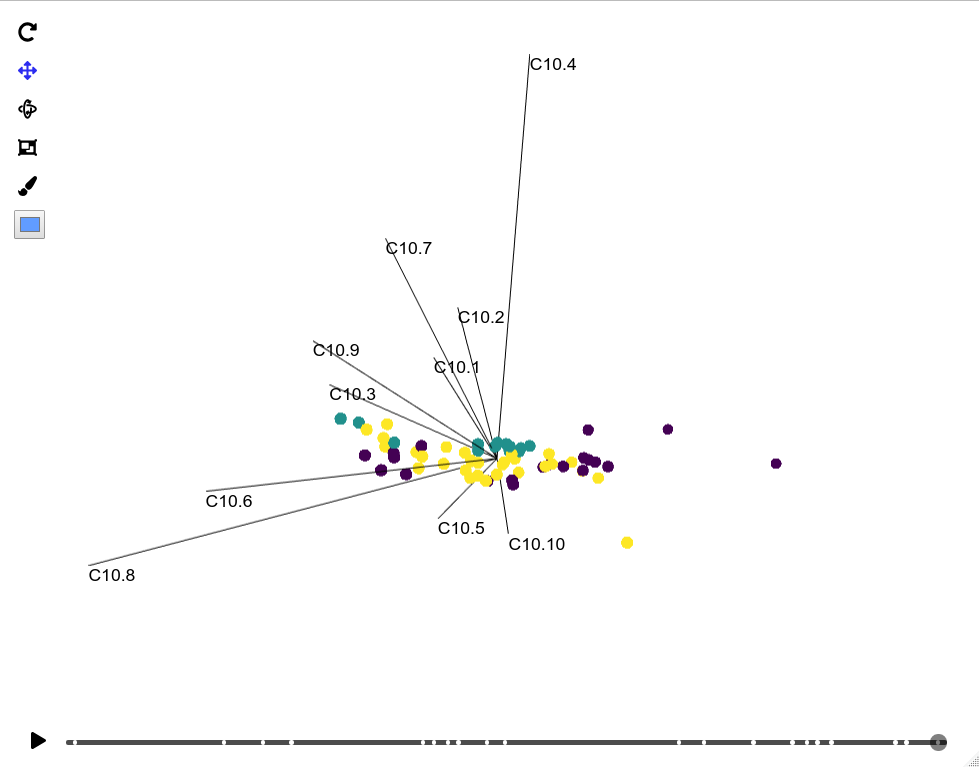
\includegraphics[scale=0.35]{spline_10.png}
	\caption{Visualization of 10th component of the Splines.}
	\label{fig:spline_10}
\end{figure}



\section{Functional Isolation Forest}
The Functional Isolation Forest method is an anomaly detection algorithm that can be used to detect the outliers in functional data. Here we have used it to detect the outliers in the Kneading data. Figure \ref{fig:kneading_outliers} shows the outliers in the Kneading data with a trim of 0.1.

\begin{figure}
	\centering
	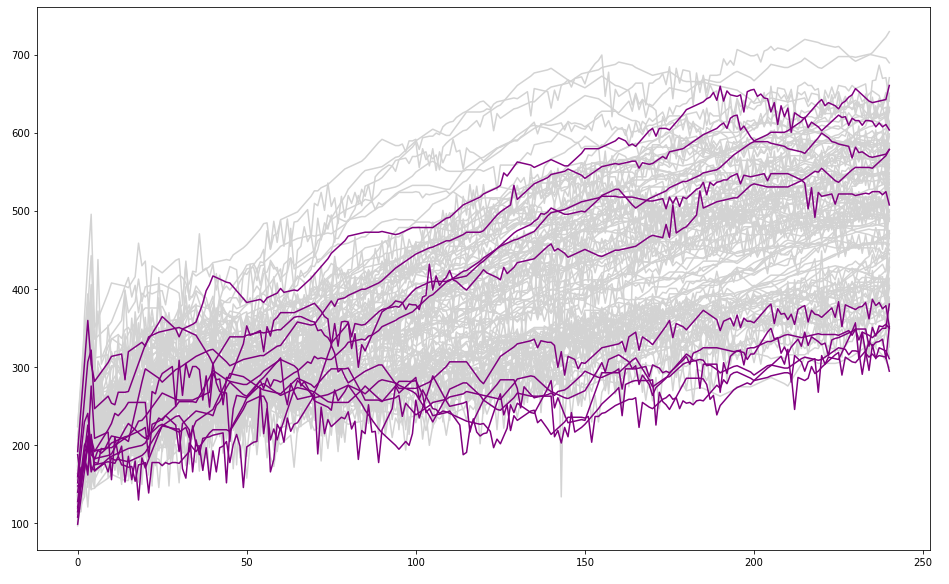
\includegraphics[scale=0.35]{kneading_outliers.png}
	\caption{Outliers in the Kneading data.}
	\label{fig:kneading_outliers}
\end{figure}

The Functional Isolation Forest algorithm can also be used to cluster data. However there are various things to consider when one is using the algorithm in such a task. There must only be two clusters/classes present in the data. Either the proportion of each class in the original datamust be known beforehand or the data must be balanced. Only when these conditions are satisfied, can the algorithm be used to cluster functional data. This is due to the fact that all the outliers detected by the algorithm are clustered into one class while the rest are clustered into another class. Thus this clustering can only be performed on the ECG data as it was made up of two classes. Before applying the algorithm, the data was undersampled into a balanced dataset. These processes helped the algorithm achieve a CCR of 76.87 on the data. Figure \ref{fig:fif_cluster} shows the clustering done by the algorithm.

\begin{figure}
	\centering
	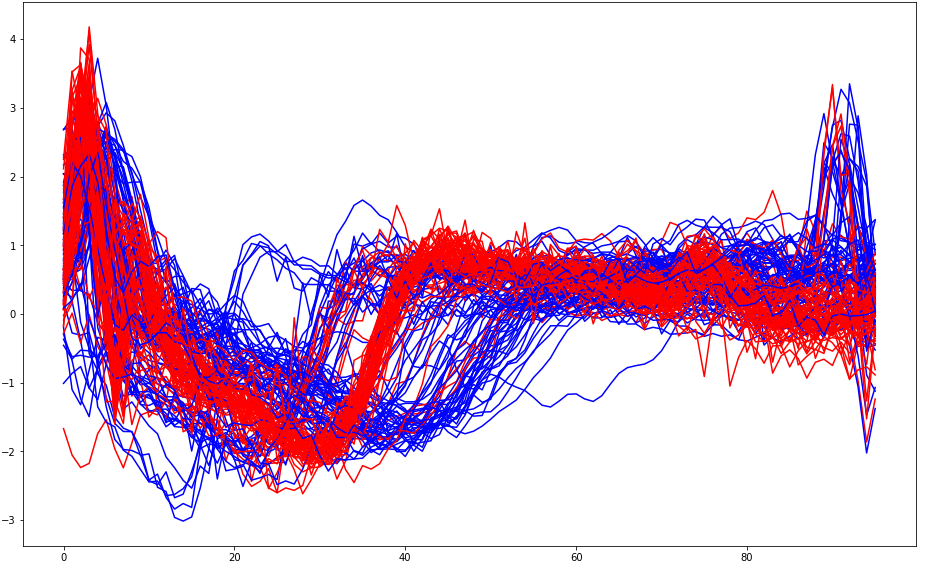
\includegraphics[scale=0.35]{fif_cluster.png}
	\caption{Clustering of the Kneading data by the FIF algorithm.}
	\label{fig:fif_cluster}
\end{figure}



\section{Conclusion}

After testing out all the algorithms on the two datasets we can say that tfunHDDC comes out ahead as the better performer in this case. This is closely followed by the cfunHDDC algorithm as it performs the same as funHDDC in the ECG data, but better in the Kneading data. Overall all algorithms are very proficient in clustering functional data. However, tfunHDDC and cfunHDDC have an edge in clustering contaminated functional data. The \emph{tourr} package is an excellent way to visualize multivariate data and would provide useful insights. Information such as the PCA component or the Spline that is able to most effectively separate the classes can be obtained by using this tool. Finally Functional Isolation Forest is a good way to determine the outliers present in a dataset. However, even though it can be used to cluster data, the sever constraints it has in doing so suggest that other techniques might fare better.



\section{Acknowledgements}
I would like to thank Mitacs for providing me with this opportunity to attend a research program in Canada. I would like to thank my supervising professor, Cristina Anton for her guidance and support throughout the course of this internship. I would also like to thank my colleague Iain Smith for his insights and tips that helped me immensely while learning about and conducting the simulations and experiments. Finally, I would like to thank the MacEwan University for providing me with the tools and office space necessary to take part in this internship.



\end{document}
